\documentclass[12pt]{article}

\usepackage[pdftex]{graphicx}
\usepackage{cancel}
\usepackage[margin=4cm]{geometry}
\usepackage[hidelinks]{hyperref}
\usepackage{fancyhdr}
\usepackage{amsmath}
\usepackage{amsfonts}
\usepackage{dirtytalk}
\usepackage{parskip}

\newcommand\tab[1][1cm]{\hspace*{#1}}
\newcommand{\HRule}{\rule{\linewidth}{0.5mm}}
\newcommand{\course}{COMS 474}

\setcounter{secnumdepth}{0} % Disable section/subsection numbering
\hyphenpenalty 10000 % Prevent words from being broken over multiple lines
\exhyphenpenalty 10000 % Prevent words from being broken over multiple lines

% Margins
\topmargin=-0.45in
\evensidemargin=0in
\oddsidemargin=0in
\textwidth=6.5in
\textheight=9.0in
\headsep=0.25in
\title{ \course \\\large Homework 7 }
\author{ Haadi Majeed }
\date{Spring 2022}


\pagestyle{fancy}
\fancyhead{}
\fancyfoot{}
\lhead{\course}
\chead{Haadi Majeed}
\rhead{Page \thepage}

\begin{document}
\maketitle
\pagebreak

% Optional TOC
%\tableofcontents
\pagebreak
\section{Problem 1}
 [30 points]\\
For this problem you will fit classifiers to three simple data-sets and visually examine the classification boundaries\\
\subsection{A}
Copy of Plot\\
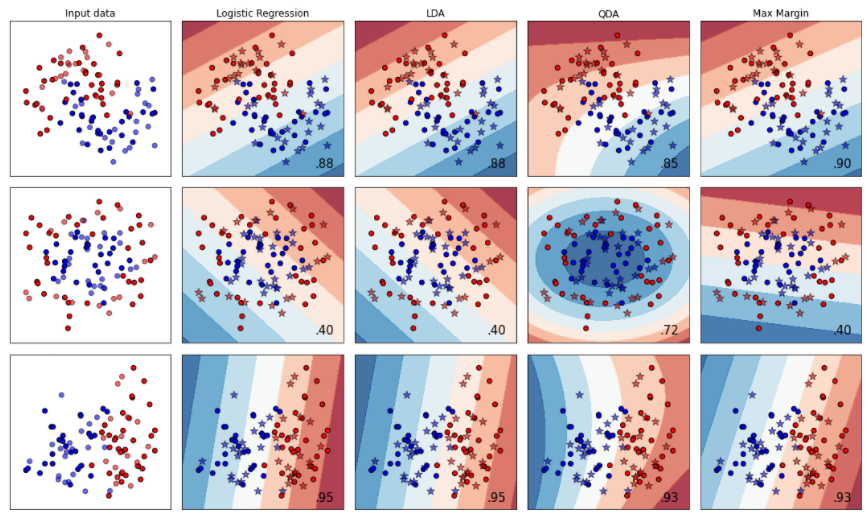
\includegraphics[width=1\textwidth]{p1.a.1.png}
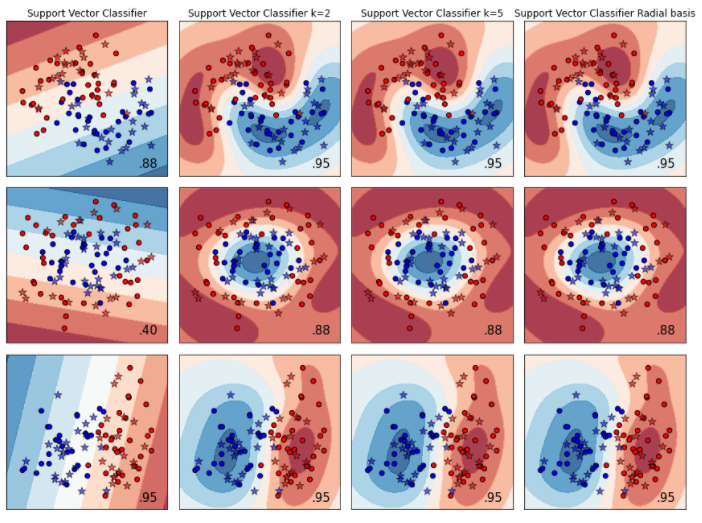
\includegraphics[width=1\textwidth]{p1.a.2.png}

\subsection{B}
Based on discussions in lecture, which methods do you expect to fit models that would result in linear decision boundaries? Was that the case? Briefly describe whether the methods that have linear boundaries appear to find the same/similar/different boundaries.\\\\
We expect that the following would have linear decision boundaries: Logistic Regression, LDA, Max Margin, SVC Linear. They mostly appear to have similar boundaries except for SVC Linear, which has the colours set differently, meaning that the predicted values would be inverted in comparison to the other models.

\subsection{C}
Repeat the same for methods known to have boundaries defined by quadratic equations.\\
QDA and the other SVCs have quadratic boundaries, which was expected behaviour since they are meant for quadratic analysis. The predictions are a bit more precise in some cases than others, but it is all as the sample data and test data see fit.

\subsection{D}
For methods whose boundaries can be non-linear, do they appear linear for the "linearly separable" data set?\\\\
Yes, it appears to look more linear-ish since the data it is fitting follows such a trend. Boundaries that are low order can be visibly seen in the models.

\subsection{E}
How do LDA and QDA compare for these data sets?\\\\
They are fairly close in this case, with QDA being a bit more flexible to the data, however in this case, that is a bad thing as QDA had a score of $.93$ vs LDA's $.95$ meaning LDA did a little bit better than QDA in this instance.

\subsection{F}
How do the different support vector methods compare?\\\\
The linear SVC scored lower for the first two data types than the quadratic SVCs except for the linearly separable data set, where the scores were equal for all 4 SVCs. For the second data set the linear SVC did significantly worse than the quadratic ones since it severely lacked the flexibility needed to fit the data properly.

%--/Paper--
\end{document}